\documentclass[12pt]{article}

\usepackage[utf8]{inputenc}
\usepackage{latexsym,amsfonts,amssymb,amsthm,amsmath}

\setlength{\parindent}{0in}
\setlength{\oddsidemargin}{0in}
\setlength{\textwidth}{6.5in}
\setlength{\textheight}{8.8in}
\setlength{\topmargin}{0in}
\setlength{\headheight}{18pt}
\usepackage{graphicx} % Required for inserting images
\usepackage{enumitem}
\usepackage{listings}
\lstset{
    basicstyle=\scriptsize\ttfamily,
    breaklines=true,
    frame=single
}

\usepackage{xcolor}

\usepackage{booktabs}

\usepackage{tikz}
\usepackage{pgfplots}
\pgfplotsset{compat=1.18}

\usepackage[toc]{appendix}

\title{Econometría 2502 - Taller 3}
\author{Rafael Marulanda y Lorena Toro}
\date{25 de octubre de 2025}

\begin{document}

\maketitle

\section{Sesgo en la estimación del efecto de un programa de capacitación laboral}

Para probar la eficacia de un programa de capacitación laboral sobre los salarios de los trabajadores, se especifica el modelo:

\[
\log(wage) = \beta_{0} + \beta_{1}train + \beta_{2}educ + \beta_{3}exper + u
\]

Donde \textit{train} es una variable binaria que es igual a uno si el trabajador participó en el programa. Considere que el término de error $u$ comprende capacidades no observadas del trabajador. Si los trabajadores con menos capacidades tienen más probabilidades de ser elegidos para participar en el programa y se emplea un análisis por MCO, ¿qué se puede decir acerca del posible sesgo en $\beta_{1}$?

\subsection*{Respuesta}

Para que la estimación por Mínimos Cuadrados Ordinarios (MCO) de $\beta_1$ sea insesgada, se requiere que $\text{Cov}(\text{train}, u) = 0$. Sin embargo, si los trabajadores con menores capacidades son más propensos a participar en el programa, y las capacidades afectan positivamente el salario (por lo que están en $u$ con signo positivo), entonces $\text{train}$ está correlacionada negativamente con $u$: $\text{Cov}(\text{train}, u) < 0$.
El sesgo en $\hat{\beta}_1$ surge de esta correlación. Dado que las capacidades más bajas implican valores más bajos de $u$ y mayor participación en el programa, el sesgo es negativo. Esto significa que $\hat{\beta}_1$ subestima el verdadero efecto causal $\beta_1$ del programa, ya que el MCO confunde el efecto del entrenamiento con la desventaja salarial inicial de los participantes con menores capacidades.

\section{Determinantes del ingreso mensual}

Un economista está investigando los determinantes del ingreso mensual (\textit{income}) de una muestra de individuos, considerando las siguientes variables explicativas:

\begin{itemize}
    \item \textbf{educ}: Años de educación formal.
    \item \textbf{exper}: Años de experiencia laboral.
    \item \textbf{female}: Variable dummy que toma el valor de 1 si la persona es mujer y 0 si es hombre.
    \item \textbf{urban}: Variable dummy que toma el valor de 1 si la persona vive en una zona urbana y 0 si vive en una zona rural.
    \item \textbf{age}: Edad del individuo (en años).
\end{itemize}

Se estiman 10 modelos de regresión lineal y se presentan sus resultados:

\begin{itemize}
    \item $income = \beta_{0} + \beta_{1}educ + u$
    \item $income = \beta_{0} + \beta_{1}educ + \beta_{2}exper + u$
    \item $income = \beta_{0} + \beta_{1}educ + \beta_{2}exper + \beta_{3}female + u$
    \item $income = \beta_{0} + \beta_{1}educ + \beta_{2}exper + \beta_{3}female + \beta_{4}urban + u$
    \item $\log(income) = \beta_{0} + \beta_{1}educ + \beta_{2}exper + \beta_{3}female + u$
    \item $income = \beta_{0} + \beta_{1}educ + \beta_{2}exper + \beta_{3}female + \beta_{4}age + \beta_{5}age^{2} + u$
    \item $income = \beta_{0} + \beta_{1}educ + \beta_{2}exper + \beta_{3}female + \beta_{4}(educ)(exper) + u$
    \item $\log(income) = \beta_{0} + \beta_{1}educ + \beta_{2}\log(exper) + \beta_{3}female + u$
    \item $income = \beta_{0} + \beta_{1}educ + \beta_{2}exper + \beta_{3}female + \beta_{4}(urban)(female) + u$
    \item $\log(income) = \beta_{0} + \beta_{1}educ + \beta_{2}exper + \beta_{3}female + \beta_{4}age + \beta_{5}age^{2} + \beta_{3}urban + u$
\end{itemize}

\subsection*{Preguntas}

\begin{enumerate}
    \item[a.] ¿Cómo se interpreta el coeficiente en el primer modelo?
    \item[b.] En el segundo modelo, ¿cómo cambia la interpretación de $\beta_{1}$ comparado con el primer modelo?
    \item[c.] En el tercer modelo, ¿cómo se interpreta el coeficiente de \textit{female}?
    \item[d.] En el cuarto modelo, ¿cómo se interpreta el coeficiente de \textit{urban}?
    \item[e.] En el quinto modelo, ¿qué significa el coeficiente de \textit{educ} dado que la variable dependiente está en logaritmo?
    \item[f.] En el sexto modelo, ¿cómo se interpreta el coeficiente asociado a $age^{2}$?
    \item[g.] En el séptimo modelo, ¿cómo se interpreta el coeficiente de la interacción $educ \times exper$?
    \item[h.] En el octavo modelo, ¿qué representa el coeficiente de $\log(exper)$?
    \item[i.] En el noveno modelo, ¿cómo se interpreta el término de interacción entre \textit{urban} y \textit{female}?
    \item[j.] En el décimo modelo, ¿cómo se interpreta el coeficiente de $age$ sobre el logaritmo del ingreso?
\end{enumerate}

\subsection*{a) Interpretación del coeficiente en el primer modelo}
En el modelo (1)
\[
income = \beta_{0} + \beta_{1}educ + u,
\]
el coeficiente $\beta_{1}$ representa el cambio esperado en el ingreso (medido en las mismas unidades que la variable \textit{income}) asociado a un año adicional de educación, manteniendo implícitamente constantes las demás determinantes que no están incluidas en el modelo. Es decir,
\[
\frac{\partial \mathbb{E}[income \mid educ]}{\partial educ} = \beta_{1}.
\]


\subsection*{b) Cambio en la interpretación de $\beta_{1}$ en el segundo modelo}
En el modelo (2)
\[
income = \beta_{0} + \beta_{1}educ + \beta_{2}exper + u,
\]
$\beta_{1}$ ahora es el efecto parcial de la educación condicionada a los años de experiencia: el cambio esperado en el ingreso por un año adicional de educación manteniendo constante la experiencia laboral. Matemáticamente,
\[
\frac{\partial \mathbb{E}[income \mid educ, exper]}{\partial educ} = \beta_{1}.
\]

\subsection*{c) Interpretación del coeficiente de \textit{female} en el tercer modelo}
En el modelo (3)
\[
income = \beta_{0} + \beta_{1}educ + \beta_{2}exper + \beta_{3}female + u,
\]
$\beta_{3}$ mide la diferencia \emph{promedio} en ingreso entre mujeres y hombres \emph{manteniendo constantes} educ y exper. Es decir, una mujer (female = 1) tiene en promedio un ingreso $\beta_{3}$ unidades mayor (si $\beta_{3}>0$) o menor (si $\beta_{3}<0$) que un hombre con los mismos años de educación y experiencia:
\[
\mathbb{E}[income \mid female=1, educ, exper] - \mathbb{E}[income \mid female=0, educ, exper] = \beta_{3}.
\]

\subsection*{d) Interpretación del coeficiente de \textit{urban} en el cuarto modelo}
En el modelo (4)
\[
income = \beta_{0} + \beta_{1}educ + \beta_{2}exper + \beta_{3}female + \beta_{4}urban + u,
\]
$\beta_{4}$ representa la diferencia promedio en ingreso entre individuos que viven en zonas urbanas y rurales, \emph{ceteris paribus} (mismos educ, exper y female). Es decir,
\[
\mathbb{E}[income \mid urban=1,\ldots] - \mathbb{E}[income \mid urban=0,\ldots] = \beta_{4}.
\]
Si $\beta_{4}>0$, vivir en zona urbana está asociado con un mayor ingreso promedio.

\subsection*{e) Significado del coeficiente de \textit{educ} en el quinto modelo (dependiente en log)}
En el modelo (5)
\[
\log(income) = \beta_{0} + \beta_{1}educ + \beta_{2}exper + \beta_{3}female + u,
\]
$\beta_{1}$ se interpreta como el cambio porcentual aproximado en el ingreso asociado a un año adicional de educación, manteniendo constantes las demás variables. Específicamente, para cambios pequeños,
\[
100\cdot \beta_{1}\ \text{\% (aprox.)}
\]
es el cambio porcentual en $income$ por un año adicional de \textit{educ}. También:
\[
 \frac{\Delta income}{income}\approx \beta_{1}.
\]
La conversión exacta entre niveles y logs para cambios discretos grandes es \(100\cdot (e^{\beta_{1}}-1)\%\).

\subsection*{f) Interpretación del coeficiente asociado a $age^{2}$ en el sexto modelo}
En el modelo (6)
\[
income = \beta_{0} + \beta_{1}educ + \beta_{2}exper + \beta_{3}female + \beta_{4}age + \beta_{5}age^{2} + u,
\]
$\beta_{5}$ captura la curvatura (no linealidad) del efecto de la edad sobre el ingreso. El efecto marginal de la edad sobre el ingreso es
\[
\frac{\partial \mathbb{E}[income]}{\partial age} = \beta_{4} + 2\beta_{5}\,age.
\]
Si $\beta_{5}<0$ la relación es cóncava (ingreso aumenta con la edad hasta un punto y luego decrece); si $\beta_{5}>0$ es convexa. El signo y magnitud de $\beta_{4}$ y $\beta_{5}$ determinan el punto de máximo/minimo cuando exista.

\subsection*{g) Interpretación del coeficiente de la interacción $educ\times exper$ en el séptimo modelo}
En el modelo (7)
\[
income = \beta_{0} + \beta_{1}educ + \beta_{2}exper + \beta_{3}female + \beta_{4}\,(educ)(exper) + u,
\]
el coeficiente de interacción $\beta_{4}$ indica que el efecto marginal de \textit{educ} sobre el ingreso depende del nivel de \textit{exper} y viceversa. Los efectos marginales son:
\[
\frac{\partial \mathbb{E}[income]}{\partial educ} = \beta_{1} + \beta_{4}\,exper,
\qquad
\frac{\partial \mathbb{E}[income]}{\partial exper} = \beta_{2} + \beta_{4}\,educ.
\]
Por ejemplo, si $\beta_{4}>0$, la ganancia en ingreso por un año adicional de educación es mayor cuanto más experiencia tiene el individuo.

\subsection*{h) Interpretación del coeficiente de $\log(exper)$ en el octavo modelo}
En el modelo (8)
\[
\log(income) = \beta_{0} + \beta_{1}educ + \beta_{2}\log(exper) + \beta_{3}female + u,
\]
$\beta_{2}$ es una elasticidad: mide el cambio porcentual en el ingreso asociado a un cambio porcentual en la experiencia. Más precisamente, si $\log(exper)$ aumenta en 1\% (es decir, exper aumenta aproximadamente 1\%), entonces $income$ cambia aproximadamente $\beta_{2}\%$. Por ejemplo, $\beta_{2}=0.2$ implica que un aumento del 1\% en \textit{exper} está asociado a un aumento aproximado del 0.2\% en \textit{income}.

\subsection*{i) Interpretación del término de interacción $urban\times female$ en el noveno modelo}
En el modelo (9)
\[
income = \beta_{0} + \beta_{1}educ + \beta_{2}exper + \beta_{3}female + \beta_{4}\,(urban)(female) + u,
\]
la interacción permite que el efecto de ser mujer difiera entre zonas urbanas y rurales. Los efectos son:
\begin{itemize}
    \item Para un individuo rural (\(urban=0\)): el efecto de ser mujer es $\beta_{3}$.
    \item Para un individuo urbano (\(urban=1\)): el efecto de ser mujer es $\beta_{3} + \beta_{4}$.
\end{itemize}
Por lo tanto, $\beta_{4}$ mide la diferencia adicional en el efecto de ser mujer cuando se pasa de rural a urbano.

\subsection*{j) Interpretación del efecto marginal de $age$ sobre $\log(income)$ en el décimo modelo}
En el modelo (10)
\[
\log(income) = \beta_{0} + \beta_{1}educ + \beta_{2}exper + \beta_{3}female + \beta_{4}age + \beta_{5}age^{2} + \beta_{6}urban + u,
\]
el efecto marginal de la edad sobre el logaritmo del ingreso es
\[
\frac{\partial \mathbb{E}[\log(income)]}{\partial age} = \beta_{4} + 2\beta_{5}\,age.
\]
Como la variable dependiente está en logaritmos, esta derivada se interpreta como el cambio proporcional (aproximado) en el ingreso asociado a un aumento de una unidad en la edad. Es decir, para una persona de edad \(age\), un año adicional de edad está asociado aproximadamente a un cambio porcentual en el ingreso de
\[
100\cdot(\beta_{4} + 2\beta_{5}\,age)\ \%.
\]

\section{Efecto del uso de marihuana sobre el salario}

Suponga que mediante una encuesta recolecta usted datos sobre salarios, educación, experiencia y género. 
Solicita también información sobre uso de la marihuana. 
La pregunta original es: ``¿Cuántas veces fumó marihuana el mes pasado?''

\begin{enumerate}[label=\textbf{\alph*.}]
    \item Dé una ecuación que permita estimar el efecto de fumar marihuana sobre el salario, controlando los demás factores. 
    La ecuación deberá permitir hacer afirmaciones como: 
    ``se estima que fumar marihuana cinco veces más al mes hace que el salario varíe $x\%$''.
    
    \item Formule una ecuación que permita probar si el uso de drogas tiene efectos diferentes sobre los salarios de hombres y mujeres. 
    ¿Cómo puede probarse que los efectos del uso de drogas no son diferentes entre hombres y mujeres?
    
    \item Suponga que considera que es mejor medir el uso de marihuana clasificando a las personas en cuatro categorías: 
    no usuario, usuario suave (1 a 5 veces por mes), usuario moderado (6 a 10 veces por mes) y usuario fuerte (más de 10 veces por mes). 
    Ahora, diseñe un modelo que permita estimar el efecto del uso de la marihuana sobre el salario.
    
    \item Usando el modelo del inciso (iii), explique detalladamente cómo probar la hipótesis nula de que fumar marihuana no tiene ningún efecto sobre el salario.
\end{enumerate}

\subsection*{a) Modelo base con consumo de marihuana}
    Una especificación adecuada es un modelo log-lineal para el salario:
    \[
    \ln(w_i) = \beta_0 + \beta_1 \, \text{Marihuana}_i + \beta_2 \, \text{Educación}_i 
    + \beta_3 \, \text{Experiencia}_i + \beta_4 \, \text{Género}_i + u_i
    \]
    donde $\ln(w_i)$ es el logaritmo del salario del individuo $i$ y 
    $\text{Marihuana}_i$ representa el número de veces que fumó marihuana en el último mes. 
    El coeficiente $\beta_1$ puede interpretarse como el cambio porcentual en el salario por una unidad adicional de consumo de marihuana. 
    Así, ``fumar cinco veces más'' se interpreta como $5\%$ de variación en el salario.

\subsection*{b) Diferencias de género}
    El modelo sería:
    \[
    \ln(w_i) = \beta_0 + \beta_1 \, \text{Marihuana}_i + \beta_2 \, \text{Género}_i 
    + \beta_3 (\text{Marihuana}_i \times \text{Género}_i) 
    + \beta_4 \, \text{Educación}_i + \beta_5 \, \text{Experiencia}_i + u_i
    \]
    donde $\text{Género}_i$ es una variable dicotómica (1 si es hombre, 0 si es mujer). 
    El coeficiente $\beta_3$ mide la diferencia en el efecto del consumo de marihuana sobre el salario entre hombres y mujeres.  
    Para probar si los efectos son iguales, se plantea la hipótesis nula:
    \[
    H_0: \beta_3 = 0
    \]
    Si no se rechaza $H_0$, entonces el efecto de la marihuana sobre el salario no difiere por género.

\subsection*{c) Modelo con categorías de consumo}
    El modelo con variables dicotómicas (dummies) es:
    \[
    \ln(w_i) = \beta_0 + \beta_1 D^{\text{suave}}_i + \beta_2 D^{\text{moderado}}_i + \beta_3 D^{\text{fuerte}}_i 
    + \beta_4 \, \text{Educación}_i + \beta_5 \, \text{Experiencia}_i + \beta_6 \, \text{Género}_i + u_i
    \]
    donde:
    \begin{itemize}
        \item $D^{\text{suave}}_i = 1$ si el individuo es usuario suave, 0 en otro caso,
        \item $D^{\text{moderado}}_i = 1$ si el individuo es usuario moderado, 0 en otro caso,
        \item $D^{\text{fuerte}}_i = 1$ si el individuo es usuario fuerte, 0 en otro caso.
    \end{itemize}
    El grupo de referencia son los no usuarios.  
    Los coeficientes $\beta_1, \beta_2, \beta_3$ representan el efecto diferencial en el salario (porcentaje) frente a los no usuarios.

\subsection*{d) Contraste de hipótesis}
    La hipótesis nula de que fumar marihuana no tiene efecto implica que los coeficientes de las tres categorías de usuarios son iguales a cero:
    \[
    H_0: \beta_1 = \beta_2 = \beta_3 = 0
    \]
    Frente a la alternativa:
    \[
    H_a: \text{al menos uno de los coeficientes es diferente de 0.}
    \]
    Para probar esta hipótesis conjunta, se utiliza un test $F$ de significancia conjunta en el modelo de regresión.  
    Si se rechaza $H_0$, concluimos que al menos una categoría de usuarios presenta un efecto significativo sobre el salario en comparación con los no usuarios.

\section{Modelo de interacción entre variable binaria y cuantitativa}

Sea $d$ una variable binaria y sea $z$ una variable cuantitativa. Considere el modelo

\[
y = \beta_{0} + \delta_{0}d + \beta_{1}z + \delta_{1}(d)(z) + u
\]

Esta es la versión general de un modelo con una interacción entre una variable binaria y una variable cuantitativa.

\subsection*{a) Funciones lineales para $d=0$ y $d=1$}
Como no se altera nada, haga el error igual a cero, $u = 0$. Entonces, cuando $d = 0$ la relación entre $y$ y $z$ puede expresarse mediante la función
\[
f_{0}(z) = \beta_{0} + \beta_{1}z.
\]
Escriba la misma relación para el caso en que $d = 1$, donde, en el lado izquierdo, debe usar $f_{1}(z)$ para denotar la función lineal de $z$. Grafique ambas funciones.

\subsection*{b) Punto de intersección de las rectas}
Suponiendo que $\delta_{1} \neq 0$ (lo que significa que las dos rectas no son paralelas), muestre que el valor $z^{*}$ para el que $f_{1}(z^{*}) = f_{0}(z^{*})$. Este es el punto en el que se interceptan las dos rectas. Argumente que $z^{*}$ es positivo si y sólo si $\delta_{1}$ y $\delta_{0}$ tienen signos contrarios.

\subsection*{c) Estimación con datos empíricos}
Empleando los datos del archivo \texttt{TWOYEAR.RAW}, puede estimarse la siguiente ecuación:

\[
\widehat{\log(wage)} = 2.289 - 0.357female + 0.50totcoll + 0.030(totcoll)(female)
\]

\[
n = 6736; \quad R^{2} = 0.202
\]

donde todos los coeficientes se han redondeado a dos cifras decimales. Empleando esta ecuación, encuentre un valor de \texttt{totcoll} (años que pasan en la universidad), tal que los valores que se predicen para $\log(wage)$ sean iguales para hombres y para mujeres.

\subsection*{d) Interpretación de los resultados}
Con base en la ecuación del inciso (iii), ¿es realmente posible que las mujeres logren suficientes años de universidad de manera que sus ingresos estén al nivel de los de los hombres? Explique.

\subsection*{a) Funciones lineales y gráfica}

Para el caso en que $d=0$, la relación entre $y$ y $z$ es:
\[
f_{0}(z) = \beta_{0} + \beta_{1}z.
\]

Para el caso en que $d=1$, la relación es:
\[
f_{1}(z) = (\beta_{0} + \delta_{0}) + (\beta_{1} + \delta_{1})z.
\]

Ambas son funciones lineales de $z$. La diferencia entre ellas depende de los parámetros $\delta_{0}$ (cambio en la ordenada al origen) y $\delta_{1}$ (cambio en la pendiente).

\vspace{0.5cm}

\begin{center}
\begin{tikzpicture}
\begin{axis}[
    axis lines=middle,
    xlabel={$z$},
    ylabel={$y$},
    xmin=0, xmax=10,
    ymin=0, ymax=15,
    legend style={at={(0.97,0.03)},anchor=south east},
    grid=both
]
% f0(z) = beta0 + beta1 z  (ejemplo: beta0=2, beta1=1)
\addplot[blue,thick,domain=0:10] {2 + 1*x};
\addlegendentry{$f_{0}(z) = \beta_{0} + \beta_{1}z$};

% f1(z) = (beta0+delta0) + (beta1+delta1) z (ejemplo: delta0=3, delta1=0.5)
\addplot[red,dashed,thick,domain=0:10] {5 + 1.5*x};
\addlegendentry{$f_{1}(z) = (\beta_{0}+\delta_{0}) + (\beta_{1}+\delta_{1})z$};

\end{axis}
\end{tikzpicture}
\end{center}

La recta azul corresponde a $f_{0}(z)$ (cuando $d=0$) y la recta roja discontinua a $f_{1}(z)$ (cuando $d=1$). La diferencia muestra los cambios en intercepto y pendiente.

\subsection*{b) Punto de intersección de las rectas}

Se tiene que
\[
f_{0}(z) = \beta_{0} + \beta_{1}z,
\]
\[
f_{1}(z) = (\beta_{0} + \delta_{0}) + (\beta_{1} + \delta_{1})z.
\]

Para hallar el punto de intersección $z^{*}$:
\[
f_{0}(z^{*}) = f_{1}(z^{*}).
\]

Es decir:
\[
\beta_{0} + \beta_{1}z^{*} \;=\; (\beta_{0} + \delta_{0}) + (\beta_{1} + \delta_{1})z^{*}.
\]

Simplificando:
\[
\beta_{0} + \beta_{1}z^{*} - \beta_{0} - \delta_{0} - \beta_{1}z^{*} - \delta_{1}z^{*} = 0,
\]
\[
- \delta_{0} - \delta_{1}z^{*} = 0,
\]
\[
z^{*} = - \frac{\delta_{0}}{\delta_{1}}.
\]

\noindent
\textbf{Interpretación de signos:}\\  
Si $\delta_{1} > 0$, entonces $z^{*} > 0$ requiere que $\delta_{0} < 0$.\\  
Si $\delta_{1} < 0$, entonces $z^{*} > 0$ requiere que $\delta_{0} > 0$.  

Por lo tanto, el punto de intersección es positivo si y sólo si $\delta_{0}$ y $\delta_{1}$ tienen signos contrarios.

\subsection*{c) Estimación con datos empíricos}

Se separan las ecuaciones para hombres y mujeres:

\[
\widehat{\log(wage)}_{male} = 2.289 + 0.50 \, totcoll,
\]
\[
\widehat{\log(wage)}_{female} = 1.932 + 0.53 \, totcoll.
\]

Suponiendo que son iguales:
\[
2.289 + 0.50\, totcoll = 1.932 + 0.53\, totcoll,
\]
\[
0.357 = 0.03\, totcoll \quad \Rightarrow \quad \, totcoll \approx 11.9.
\]

Por lo tanto, se necesitarían cerca de 12 años de universidad para que los salarios predichos de hombres y mujeres fueran iguales.

\subsection*{d) Interpretación de los resultados}

De acuerdo con el modelo estimado, para que los ingresos predichos de las mujeres se igualen a los de los hombres, se necesitarían alrededor de 12 años de estudios universitarios. 

En la práctica, tal cantidad de años en la universidad es irrealista, ya que la formación universitaria no pasa de 6 años en general. Esto implica que, aun cuando las mujeres incrementen su nivel educativo, el modelo predice que sus salarios esperados seguirán siendo menores que los de los hombres.

La brecha salarial entre hombres y mujeres no puede explicarse únicamente por diferencias en los años de educación. Más bien, refleja factores estructurales del mercado laboral, incluyendo formas de discriminación que no se capturan con las variables observadas.

\section{Efecto del programa de vales escolares}

Dado un niño $i$ que vive en un determinado distrito escolar, sea $voucher_i$ una variable binaria que sea igual a uno si el niño es elegido para participar en un programa de vales escolares, y sea $score_i$ la puntuación del niño en un examen estandarizado subsecuente. Suponga que la variable de participación $voucher_i$ es completamente aleatorizada en el sentido de que es independiente, tanto de los factores observados como de los no observados que pueden afectar la puntuación del examen.

\begin{enumerate}[label=\alph*)]
    \item Si corre una regresión simple de $score_i$ sobre $voucher_i$ empleando una muestra aleatoria de tamaño $n$, ¿proporciona el estimador de MCO un estimador insesgado del efecto del programa de vales?

    \item Suponga que logra obtener información adicional sobre antecedentes del niño, tales como ingreso familiar, estructura familiar (por ejemplo, si el niño vive con sus padres) y nivel de educación de los padres. ¿Necesita controlar estos factores para obtener un estimador insesgado de los efectos del programa de vales? Explique.

    \item ¿Cuál es la razón para incluir en la regresión las variables sobre los antecedentes familiares? ¿Hay alguna situación en la que usted no incluiría tales variables?
\end{enumerate}

\subsection*{a) ¿El estimador de MCO es insesgado?}
Considere la regresión lineal simple
\[
score_i = \alpha + \beta\,voucher_i + u_i.
\]
Bajo la hipótesis de aleatorización completa tenemos
\[
E[u_i \mid voucher_i] = E[u_i],
\]
es decir, $voucher_i$ es independiente del término de error que recoge todos los determinantes no modelados de $score_i$. Entonces
\[
\operatorname{Cov}(voucher_i, u_i)=0
\]
y por lo tanto el estimador de MCO para $\beta$ es insesgado:
\[
E[\hat\beta_{\text{MCO}}]=\beta.
\]
Intuitivamente, la aleatorización garantiza que las diferencias medias en $score$ entre tratados y no tratados se deben únicamente al tratamiento.

\subsection*{b) ¿Es necesario controlar antecedentes (ingreso, estructura familiar, educación de padres) para obtener un estimador insesgado?}
No es necesario para obtener un estimador insesgado. Debido a la aleatorización, $voucher_i$ es independiente de las covariables observadas y no observadas en expectativa, por lo que el estimador de MCO sin controles ya es insesgado.

\subsection*{c) ¿Por qué incluir las variables de antecedentes? ¿Cuándo no incluirlas?}
\textbf{Razones para incluirlas}

Si la aleatorización se hizo estratificando (por escuela, por barrio, etc.), es correcto incluir las variables de estratificación o efectos fijos correspondientes para obtener estimadores con varianzas adecuadas.

\textbf{Situaciones para no incluirlas}

No se debe controlar por variables que son consecuencias del tratamiento, porque condicionarlas puede inducir sesgo (p.\,ej. variables que cambian como resultado de recibir el voucher).

\section{Determinantes del salario}

Para este ejercicio emplee los datos del archivo \texttt{WAGE2.RAW}.

\subsection*{a.}
Estime el modelo:
\[
\log(wage) = \beta_0 + \beta_1 educ + \beta_2 exper + \beta_3 tenure + \beta_4 married + \beta_5 black + \beta_6 south + \beta_7 urban + u
\]

y dé el resultado en la forma habitual. Manteniendo todos los demás factores constantes, ¿cuál es la diferencia aproximada entre el salario mensual de negros y no negros? 
¿Es esta diferencia estadísticamente significativa?

\subsection*{b.}
Agregue a esta ecuación las variables $exper^2$ y $tenure^2$ y muestre que no son conjuntamente significativas al nivel de 20\%.

\subsection*{c.}
Amplíe el modelo original de manera que el rendimiento a la educación dependa de la raza y pruebe si en realidad el rendimiento de la educación depende de la raza.

\subsection*{d.}
Partiendo nuevamente del modelo original, permita que los salarios difieran entre cuatro grupos: casados negros, casados no negros, solteros negros y solteros no negros. 
¿Cuál es la diferencia de salario estimada entre negros casados y no negros casados?

\subsection*{a. Estimación del modelo}

El modelo estimado por Mínimos Cuadrados Ordinarios (MCO) es:

\begin{equation}
\widehat{\log(wage)} = 5.3955 + 0.0654 \, \text{educ} + 0.0140 \, \text{exper} + 0.0117 \, \text{tenure} + 0.1994 \, \text{married} - 0.1883 \, \text{black} - 0.0909 \, \text{south} + 0.1839 \, \text{urban}
\end{equation}

Los resultados detallados de la regresión son los siguientes:

\begin{table}[h]
\centering
\begin{tabular}{lccccc}
\toprule
Variable & Coeficiente & Error estándar & t-stat & p-valor & Intervalo de confianza al 95\% \\
\midrule
educ     & 0.0654 & 0.0063 & 10.47 & 0.000 & [0.0532, 0.0777] \\
exper    & 0.0140 & 0.0032 & 4.41  & 0.000 & [0.0078, 0.0203] \\
tenure   & 0.0117 & 0.0025 & 4.79  & 0.000 & [0.0069, 0.0166] \\
married  & 0.1994 & 0.0391 & 5.11  & 0.000 & [0.1228, 0.2761] \\
black    & -0.1883 & 0.0377 & -5.00 & 0.000 & [-0.2623, -0.1144] \\
south    & -0.0909 & 0.0262 & -3.46 & 0.001 & [-0.1424, -0.0394] \\
urban    & 0.1839 & 0.0270 & 6.82  & 0.000 & [0.1310, 0.2368] \\
\_cons   & 5.3955 & 0.1132 & 47.65 & 0.000 & [5.1733, 5.6177] \\
\bottomrule
\end{tabular}
\caption{Resultados de la regresión para el modelo log(wage)}
\end{table}

\begin{itemize}
    \item Número de observaciones: 935
    \item \( F(7, 927) = 44.75 \) (Prob \( > F = 0.0000 \))
    \item \( R^2 = 0.2526 \)
    \item \( R^2 \) ajustado = 0.2469
    \item Raíz del ECM = 0.3655
\end{itemize}

Manteniendo constantes las demás variables (educación, experiencia, antigüedad, estado civil, región sur y residencia urbana), la diferencia aproximada en el salario mensual entre negros y no negros se deriva del coeficiente de la variable dummy \textit{black}. Dado que el modelo es semilogarítmico, el efecto porcentual aproximado es \( 100 \times \hat{\beta}_5 = 100 \times (-0.1883) \approx -18.83\% \). Esto implica que, ceteris paribus, los negros tienen un salario mensual aproximadamente 18.8\% menor que los no negros.

Esta diferencia es estadísticamente significativa, ya que el estadístico $ t = -5.00 $ con un p-valor de 0.000 permite rechazar la hipótesis nula de que el coeficiente es cero al nivel de significancia convencional.

\subsection*{b. Inclusión de $exper^2$ y $tenure^2$}

El modelo ampliado con las variables $exper^2$ y $tenure^2$ es:

\[
\widehat{\log(wage)} = 5.3587 + 0.0643 \, educ + 0.0172 \, exper - 0.0001 \, exper^2 + 0.0249 \, tenure - 0.0008 \, tenure^2 + 0.1985 \, married - 0.1907 \, black - 0.0912 \, south + 0.1854 \, urban
\]

Los resultados de la regresión son los siguientes:

\begin{center}
\begin{tabular}{lccccc}
\hline
Variable & Coeficiente & Error estándar & $t$-stat & $p$-valor & Intervalo de confianza (95\%) \\
\hline
$educ$ & 0.0643 & 0.0063 & 10.18 & 0.000 & [0.0519, 0.0767] \\
$exper$ & 0.0172 & 0.0126 & 1.36 & 0.173 & [-0.0075, 0.0420] \\
$exper^2$ & -0.0001 & 0.0005 & -0.21 & 0.831 & [-0.0012, 0.0009] \\
$tenure$ & 0.0249 & 0.0081 & 3.07 & 0.002 & [0.0090, 0.0409] \\
$tenure^2$ & -0.0008 & 0.0005 & -1.69 & 0.091 & [-0.0017, 0.0001] \\
$married$ & 0.1985 & 0.0391 & 5.08 & 0.000 & [0.1218, 0.2753] \\
$black$ & -0.1907 & 0.0377 & -5.06 & 0.000 & [-0.2647, -0.1167] \\
$south$ & -0.0912 & 0.0262 & -3.48 & 0.001 & [-0.1427, -0.0397] \\
$urban$ & 0.1854 & 0.0270 & 6.88 & 0.000 & [0.1325, 0.2383] \\
$\_cons$ & 5.3587 & 0.1259 & 42.56 & 0.000 & [5.1116, 5.6058] \\
\hline
\end{tabular}
\end{center}

Número de observaciones: 935 \\
$F(9, 925) = 35.17$, Prob $> F = 0.0000$ \\
$R^2 = 0.2550$, $R^2$ ajustado = 0.2477 \\
Raíz del ECM = 0.3653

Para determinar si las variables $exper^2$ y $tenure^2$ son conjuntamente significativas al nivel del 20\%, se realiza un test $F$ de la hipótesis nula:

\[
H_0: \beta_{exper^2} = \beta_{tenure^2} = 0
\]

El resultado del test $F$ es:

\[
F(2, 925) = 1.49, \quad \text{Prob} > F = 0.2260
\]

Dado que el valor $p = 0.2260$ es mayor que el nivel de significancia del 20\% ($\alpha = 0.20$), no se rechaza la hipótesis nula. Por lo tanto, las variables $exper^2$ y $tenure^2$ no son conjuntamente significativas al nivel del 20\%, lo que sugiere que los términos cuadráticos no aportan significativamente al modelo en comparación con el modelo original.

\subsection*{c. Rendimiento a la educación según raza}

Para evaluar si el rendimiento de la educación sobre el salario depende de la raza, se amplía el modelo original incluyendo un término de interacción entre \textit{educ} y \textit{black}:

\[
\log(wage) = \beta_0 + \beta_1 educ + \beta_2 exper + \beta_3 tenure + \beta_4 married + \beta_5 black + \beta_6 south + \beta_7 urban + \beta_8 (black \times educ) + u
\]

El modelo estimado por Mínimos Cuadrados Ordinarios (MCO) es:

\[
\widehat{\log(wage)} = 5.3748 + 0.0671 \, educ + 0.0138 \, exper + 0.0118 \, tenure + 0.1989 \, married + 0.0948 \, black - 0.0894 \, south + 0.1839 \, urban - 0.0226 \, (black \times educ)
\]

Los resultados de la regresión son:

\begin{center}
\begin{tabular}{l c c c c c}
\hline
Variable & Coeficiente & Error estándar & t-stat & p-valor & Intervalo de confianza (95\%) \\
\hline
educ & 0.0671 & 0.0064 & 10.44 & 0.000 & [0.0545, 0.0797] \\
exper & 0.0138 & 0.0032 & 4.33 & 0.000 & [0.0076, 0.0201] \\
tenure & 0.0118 & 0.0025 & 4.81 & 0.000 & [0.0070, 0.0166] \\
married & 0.1989 & 0.0390 & 5.09 & 0.000 & [0.1223, 0.2755] \\
black & 0.0948 & 0.2554 & 0.37 & 0.711 & [-0.4064, 0.5960] \\
south & -0.0894 & 0.0263 & -3.40 & 0.001 & [-0.1410, -0.0379] \\
urban & 0.1839 & 0.0270 & 6.82 & 0.000 & [0.1310, 0.2368] \\
black\_educ & -0.0226 & 0.0202 & -1.12 & 0.263 & [-0.0622, 0.0170] \\
\_cons & 5.3748 & 0.1147 & 46.86 & 0.000 & [5.1497, 5.5999] \\
\hline
\end{tabular}
\end{center}

Número de observaciones: 935 \\
F(8, 926) = 39.32 (Prob > F = 0.0000) \\
R-cuadrado = 0.2536 \\
R-cuadrado ajustado = 0.2471 \\
Raíz del ECM = 0.3654

El rendimiento de la educación sobre el salario es \(\beta_1 + \beta_8 \cdot black\). Para no negros (\textit{black} = 0), el rendimiento es \(\hat{\beta}_1 = 0.0671\), lo que implica un aumento aproximado de 6.71\% en el salario por año adicional de educación. Para negros (\textit{black} = 1), el rendimiento es \(\hat{\beta}_1 + \hat{\beta}_8 = 0.0671 - 0.0226 = 0.0445\), equivalente a un aumento aproximado de 4.45\% por año adicional de educación.

Para probar si el rendimiento de la educación depende de la raza, se evalúa la hipótesis nula:

\[
H_0: \beta_8 = 0 \quad (\text{el rendimiento de la educación es igual para negros y no negros})
\]

El test \(F\) para \(\hat{\beta}_8 = -0.0226\) arroja:

\[
F(1, 926) = 1.26, \quad \text{Prob} > F = 0.2626
\]

Dado que el valor \(p = 0.2626\) es mayor que los niveles de significancia convencionales (e.g., 0.05 o 0.10), no se rechaza \(H_0\). Por lo tanto, no hay evidencia estadística suficiente para concluir que el rendimiento de la educación sobre el salario difiere significativamente entre negros y no negros.

\subsection*{d. Diferencias salariales por grupos de estado civil y raza}

% Specifying the extended model
Para permitir que los salarios difieran entre los cuatro grupos (casados negros, casados no negros, solteros negros y solteros no negros), se amplía el modelo original incluyendo un término de interacción entre \textit{married} y \textit{black}:

\[
\log(wage) = \beta_0 + \beta_1 educ + \beta_2 exper + \beta_3 tenure + \beta_4 married + \beta_5 black + \beta_6 (married \times black) + \beta_7 south + \beta_8 urban + u
\]

% Describing group differences
Este modelo captura las diferencias de la siguiente manera:
\begin{itemize}
    \item Para no negros solteros (\textit{married}=0, \textit{black}=0): referencia base.
    \item Para no negros casados (\textit{married}=1, \textit{black}=0): efecto de \(\beta_4\).
    \item Para negros solteros (\textit{married}=0, \textit{black}=1): efecto de \(\beta_5\).
    \item Para negros casados (\textit{married}=1, \textit{black}=1): efecto de \(\beta_4 + \beta_5 + \beta_6\).
\end{itemize}

% Presenting the estimated model
El modelo estimado por Mínimos Cuadrados Ordinarios (MCO) es:

\[
\widehat{\log(wage)} = 5.4038 + 0.0655 \, educ + 0.0141 \, exper + 0.0117 \, tenure + 0.1889 \, married - 0.2408 \, black + 0.0614 \, (married \times black) - 0.0920 \, south + 0.1844 \, urban
\]

% Displaying regression results
Los resultados de la regresión son:

\begin{center}
\begin{tabular}{l c c c c c}
\hline
Variable & Coeficiente & Error estándar & t-stat & p-valor & Intervalo de confianza (95\%) \\
\hline
educ & 0.0655 & 0.0063 & 10.47 & 0.000 & [0.0532, 0.0777] \\
exper & 0.0141 & 0.0032 & 4.43 & 0.000 & [0.0079, 0.0204] \\
tenure & 0.0117 & 0.0025 & 4.74 & 0.000 & [0.0068, 0.0165] \\
married & 0.1889 & 0.0429 & 4.41 & 0.000 & [0.1048, 0.2731] \\
black & -0.2408 & 0.0960 & -2.51 & 0.012 & [-0.4293, -0.0524] \\
married\_black & 0.0614 & 0.1033 & 0.59 & 0.553 & [-0.1413, 0.2640] \\
south & -0.0920 & 0.0263 & -3.49 & 0.001 & [-0.1436, -0.0403] \\
urban & 0.1844 & 0.0270 & 6.83 & 0.000 & [0.1314, 0.2373] \\
\_cons & 5.4038 & 0.1141 & 47.35 & 0.000 & [5.1798, 5.6278] \\
\hline
\end{tabular}
\end{center}

Número de observaciones: 935 \\
F(8, 926) = 39.17 (Prob > F = 0.0000) \\
R-cuadrado = 0.2528 \\
R-cuadrado ajustado = 0.2464 \\
Raíz del ECM = 0.3656

% Calculating wage difference
La diferencia estimada en el salario entre negros casados y no negros casados, manteniendo constantes las demás variables, se obtiene combinando los coeficientes \(\hat{\beta}_5 + \hat{\beta}_6 = -0.2408 + 0.0614 = -0.1795\). Dado que el modelo es semilogarítmico, esta diferencia implica que los negros casados tienen un salario aproximadamente 17.95\% menor que los no negros casados (\(100 \times (-0.1795) \% \approx -18\%\)).

% Assessing statistical significance
Esta diferencia es estadísticamente significativa, ya que el estadístico t es -4.43 con un p-valor de 0.000, permite rechazar la hipótesis nula de que la diferencia es cero.

\section{Diferencias de Género en la Duración del Sueño}
Para este ejercicio use la base de datos \texttt{SLEEP75.RAW}. 
La ecuación de interés es:
\[
sleep = \beta_{0} + \beta_{1}totwrk + \beta_{2}educ + \beta_{3}age + \beta_{4}age^{2} + \beta_{5}yngkid + u
\]

\begin{enumerate}[label=\alph*)]
    \item Estime esta ecuación por separado para hombres y mujeres y dé los resultados de la manera habitual. 
    ¿Hay diferencias importantes entre las dos ecuaciones estimadas?

    \item Investigue ¿qué es la prueba de Chow? ¿En qué casos puede usarse? 
    ¿Cómo es su estadístico de prueba? Sea detallado en su investigación.

    \item Realice la prueba de Chow para la igualdad entre los parámetros para hombres y mujeres en la ecuación del sueño. 
    Utilice la forma de la prueba en la que se agrega \texttt{male} (hombre) y los términos de interacción 
    \texttt{maletotwrk}, \ldots, \texttt{maleyngkid}, y se usa el conjunto completo de observaciones. 
    ¿Cuáles son los grados de libertad pertinentes en esta prueba? 
    ¿Debe rechazarse la hipótesis nula al nivel de significancia del 5\%?

    \item Ahora tome en consideración interceptos diferentes entre hombres y mujeres y determine si los términos de interacción en los que aparece \texttt{male} son conjuntamente significativos.

    \item Dados los resultados de los incisos i), ii) y iii), ¿cuál es el modelo final?
\end{enumerate}

\subsection*{a. Estimaciones separadas por género}

% Defining the plan: Present the estimated model for men
La ecuación estimada para hombres (n=400) por Mínimos Cuadrados Ordinarios (MCO) es:

\[
\widehat{sleep} = 3648.208 - 0.1821 \, totwrk - 13.0524 \, educ + 7.1566 \, age - 0.0448 \, age^2 + 60.3802 \, yngkid
\]

% Defining the plan: Display regression results for men in a table
Los resultados detallados son:

\begin{center}
\begin{tabular}{l c c c c c}
\toprule
Variable & Coeficiente & Error estándar & t-stat & p-valor & Intervalo de confianza (95\%) \\
\midrule
totwrk & -0.1821 & 0.0245 & -7.44 & 0.000 & [-0.2303, -0.1340] \\
educ & -13.0524 & 7.4142 & -1.76 & 0.079 & [-27.6288, 1.5240] \\
age & 7.1566 & 14.3204 & 0.50 & 0.618 & [-20.9973, 35.3105] \\
age² & -0.0448 & 0.1684 & -0.27 & 0.791 & [-0.3759, 0.2863] \\
yngkid & 60.3802 & 59.0228 & 1.02 & 0.307 & [-55.6588, 176.4192] \\
\_cons & 3648.208 & 310.0393 & 11.77 & 0.000 & [3038.6700, 4257.7470] \\
\bottomrule
\end{tabular}
\end{center}

% Defining the plan: Provide regression diagnostics for men
Número de observaciones: 400 \\
F(5, 394) = 14.59 (Prob > F = 0.0000) \\
R-cuadrado = 0.1562 \\
R-cuadrado ajustado = 0.1455 \\
Raíz del ECM = 402.29

% Defining the plan: Present the estimated model for women
La ecuación estimada para mujeres (n=306) es:

\[
\widehat{sleep} = 4238.729 - 0.1399 \, totwrk - 10.2051 \, educ - 30.3566 \, age + 0.3679 \, age^2 - 118.2826 \, yngkid
\]

% Defining the plan: Display regression results for women in a table
Los resultados detallados son:

\begin{center}
\begin{tabular}{l c c c c c}
\toprule
Variable & Coeficiente & Error estándar & t-stat & p-valor & Intervalo de confianza (95\%) \\
\midrule
totwrk & -0.1399 & 0.0277 & -5.06 & 0.000 & [-0.1944, -0.0855] \\
educ & -10.2051 & 9.5888 & -1.06 & 0.288 & [-29.0751, 8.6648] \\
age & -30.3566 & 18.5309 & -1.64 & 0.102 & [-66.8236, 6.1105] \\
age² & 0.3679 & 0.2233 & 1.65 & 0.101 & [-0.0716, 0.8075] \\
yngkid & -118.2826 & 93.1876 & -1.27 & 0.205 & [-301.6667, 65.1015] \\
\_cons & 4238.729 & 384.8923 & 11.01 & 0.000 & [3481.2990, 4996.1600] \\
\bottomrule
\end{tabular}
\end{center}

% Defining the plan: Provide regression diagnostics for women
Número de observaciones: 306 \\
F(5, 300) = 6.50 (Prob > F = 0.0000) \\
R-cuadrado = 0.0977 \\
R-cuadrado ajustado = 0.0826 \\
Raíz del ECM = 436.99

% Defining the plan: Discuss key differences between the estimated equations
Existen diferencias importantes entre las ecuaciones estimadas para hombres y mujeres. El intercepto es notablemente mayor para mujeres (4238.729 vs. 3648.208), lo que sugiere que, en promedio, las mujeres duermen más cuando las variables explicativas son cero. El efecto de \textit{totwrk} es negativo y significativo en ambos grupos, pero más pronunciado en hombres (-0.1821 vs. -0.1399). Para \textit{educ}, el coeficiente es negativo en ambos, pero solo marginalmente significativo en hombres (p=0.079) y no significativo en mujeres (p=0.288). Los efectos de \textit{age} y \textit{age²} difieren en signo: para hombres, \textit{age} es positivo (aunque no significativo) y \textit{age²} negativo (no significativo), sugiriendo una relación cóncava posible; para mujeres, \textit{age} es negativo (p=0.102) y \textit{age²} positivo (p=0.101), indicando una relación convexa. El efecto de \textit{yngkid} también cambia de signo: positivo (no significativo) en hombres y negativo (no significativo) en mujeres. Además, el R-cuadrado es mayor para hombres (0.1562 vs. 0.0977), indicando que el modelo explica una mayor proporción de la varianza en el sueño para hombres.

\subsection*{b. La Prueba de Chow}

% Defining the plan: Define the Chow test and its purpose
La prueba de Chow evalúa si los coeficientes de un modelo de regresión lineal son iguales para dos subgrupos de datos, detectando posibles quiebres estructurales en la relación entre variables. Se utiliza para determinar si un modelo único es adecuado o si se requieren modelos separados para cada grupo.

% Defining the plan: Specify when the Chow test can be used
\subsubsection*{Casos en los que puede usarse}
La prueba de Chow es aplicable en los siguientes contextos:
\begin{itemize}
    \item \textbf{Series temporales}: Detectar cambios en los parámetros tras un evento conocido, como una crisis económica o un cambio de política.
    \item \textbf{Evaluación de políticas o programas}: Comparar el impacto de variables explicativas en subgrupos (e.g., hombres vs. mujeres, tratados vs. no tratados).
    \item \textbf{Estabilidad paramétrica}: Verificar si los parámetros son consistentes entre grupos (e.g., regiones o cohortes).
\end{itemize}
No es adecuada si el punto de quiebre es desconocido (se requieren tests como Quandt-Andrews) o si las submuestras son muy pequeñas (menor al número de parámetros), lo que puede generar resultados poco confiables.

% Defining the plan: Describe the test statistic and its formulation
\subsubsection*{Estadístico de prueba}
Consideremos un modelo de regresión lineal:

\[
y_i = \beta_0 + \beta_1 x_{1i} + \beta_2 x_{2i} + \dots + \beta_k x_{ki} + u_i
\]

La muestra de tamaño \( N = N_1 + N_2 \) se divide en dos subgrupos con \( k \) parámetros (incluyendo el intercepto). La hipótesis nula (\( H_0 \)) es que los coeficientes son iguales en ambos grupos. Se estiman tres modelos:
\begin{itemize}
    \item Modelo combinado (toda la muestra): suma de cuadrados residual (SSR) = \( S_C \).
    \item Modelo para el grupo 1: SSR = \( S_1 \).
    \item Modelo para el grupo 2: SSR = \( S_2 \).
\end{itemize}

El estadístico de Chow es:

\[
F = \frac{(S_C - (S_1 + S_2)) / k}{(S_1 + S_2) / (N_1 + N_2 - 2k)}
\]

donde el numerador mide el aumento en el error al asumir parámetros iguales, y el denominador es el error promedio de los modelos separados. Bajo \( H_0 \), el estadístico sigue una distribución \( F(k, N_1 + N_2 - 2k) \). Si \( F \) excede el valor crítico de la distribución \( F \), se rechaza \( H_0 \), indicando un quiebre estructural.

% Defining the plan: Explain the alternative dummy variable approach
Una formulación alternativa usa un modelo combinado con una variable dummy para el segundo grupo y términos de interacción con todas las variables explicativas. Un test \( F \) sobre la significancia conjunta de la dummy y las interacciones es equivalente a la prueba de Chow.

% Defining the plan: List assumptions
\subsubsection*{Supuestos}
\begin{itemize}
    \item Los errores \( u_i \) son independientes, idénticamente distribuidos y normales con varianza constante entre grupos.
    \item El punto de quiebre debe ser conocido ex ante.
    \item Cada submuestra debe tener al menos \( k+1 \) observaciones.
    \item El modelo es lineal y no presenta multicolinealidad perfecta.
    \item Para muestras grandes, la normalidad de los errores es menos crítica debido al teorema central del límite.
\end{itemize}

% Defining the plan: Provide illustrative examples
\subsubsection*{Ejemplos}
\begin{itemize}
    \item En series temporales, probar si los determinantes del PIB cambiaron tras una crisis económica.
    \item En un modelo de duración del sueño, verificar si los efectos de las horas de trabajo difieren entre hombres y mujeres.
    \item En evaluación de políticas, comparar el impacto de la educación en los salarios entre regiones urbanas y rurales.
\end{itemize}

\subsubsection*{Aplicación}

Examinar el impacto económico de los sistemas de recuperación de calor en operaciones de minería de Bitcoin; se usan datos mensuales de una granja minera al implementar tecnología para reutilizar el calor residual en enfriamiento por adsorción. El modelo de regresión estima las ganancias mensuales en función de costos energéticos, tasa de hash y precio de Bitcoin; con la prueba de Chow se verificaría si se rechaza la hipótesis nula de estabilidad paramétrica para confirmar que la recuperación de calor induce un quiebre estructural que mejora la rentabilidad y sostenibilidad en la minería de Bitcoin.

% Defining the plan: Conclude with a summary
La prueba de Chow es una herramienta clave en econometría para detectar cambios estructurales, pero su validez depende del cumplimiento de sus supuestos y de la especificación adecuada del punto de quiebre.

\subsection*{c. Prueba de Chow para igualdad de parámetros por género}

% Defining the plan: Present the augmented model with dummy and interaction terms
Para realizar la prueba de Chow utilizando la aproximación con variables dummy, se estima el modelo ampliado en la muestra completa (n=706), incluyendo la dummy \textit{male} (1 para hombres, 0 para mujeres) y sus interacciones con cada regresor:

\[
sleep = \beta_0 + \beta_1 totwrk + \beta_2 educ + \beta_3 age + \beta_4 age^2 + \beta_5 yngkid + \beta_6 male + \beta_7 (male \times totwrk) + \beta_8 (male \times educ) + \beta_9 (male \times age) + \beta_{10} (male \times age^2) + \beta_{11} (male \times yngkid) + u
\]

% Defining the plan: Provide the estimated regression equation
El modelo estimado por Mínimos Cuadrados Ordinarios (MCO) es:

\[
\widehat{sleep} = 4238.729 - 0.1399 \, totwrk - 10.2051 \, educ - 30.3566 \, age + 0.3679 \, age^2 - 118.2826 \, yngkid - 590.5211 \, male - 0.0422 \, (male \times totwrk) - 2.8472 \, (male \times educ) + 37.5132 \, (male \times age) - 0.4127 \, (male \times age^2) + 178.6628 \, (male \times yngkid)
\]

% Defining the plan: Display regression results in a table
Los resultados de la regresión son:

\begin{center}
\begin{tabular}{l c c c c c}
\toprule
Variable & Coeficiente & Error estándar & t-stat & p-valor & Intervalo de confianza (95\%) \\
\midrule
totwrk & -0.1399 & 0.0264 & -5.29 & 0.000 & [-0.1919, -0.0880] \\
educ & -10.2051 & 9.1643 & -1.11 & 0.266 & [-28.1983, 7.7880] \\
age & -30.3566 & 17.7105 & -1.71 & 0.087 & [-65.1291, 4.4160] \\
agesq & 0.3679 & 0.2135 & 1.72 & 0.085 & [-0.0511, 0.7870] \\
yngkid & -118.2826 & 89.0619 & -1.33 & 0.185 & [-293.1456, 56.5805] \\
male & -590.5211 & 488.7916 & -1.21 & 0.227 & [-1550.2090, 369.1665] \\
male\_totwrk & -0.0422 & 0.0367 & -1.15 & 0.251 & [-0.1142, 0.0298] \\
male\_educ & -2.8472 & 11.9680 & -0.24 & 0.812 & [-26.3450, 20.6505] \\
male\_age & 37.5132 & 23.1233 & 1.62 & 0.105 & [-7.8869, 82.9132] \\
male\_agesq & -0.4127 & 0.2759 & -1.50 & 0.135 & [-0.9544, 0.1290] \\
male\_yngkid & 178.6628 & 108.1051 & 1.65 & 0.099 & [-33.5895, 390.9150] \\
\_cons & 4238.729 & 367.8519 & 11.52 & 0.000 & [3516.4930, 4960.9650] \\
\bottomrule
\end{tabular}
\end{center}

% Defining the plan: Provide regression diagnostics
Número de observaciones: 706 \\
F(11, 694) = 9.48 (Prob > F = 0.0000) \\
R-cuadrado = 0.1306 \\
R-cuadrado ajustado = 0.1168 \\
Raíz del ECM = 417.64

% Defining the plan: Conduct the Chow test and interpret results
La hipótesis nula de la prueba de Chow es que todos los coeficientes son iguales entre hombres y mujeres, lo que equivale a probar la significancia conjunta de la dummy \textit{male} y las cinco interacciones (\( H_0: \beta_6 = \beta_7 = \beta_8 = \beta_9 = \beta_{10} = \beta_{11} = 0 \)). El resultado del test F es:

\[
F(6, 694) = 2.12, \quad \text{Prob} > F = 0.0495
\]

% Defining the plan: Specify degrees of freedom
Los grados de libertad pertinentes son 6 (número de restricciones, es decir, coeficientes probados) en el numerador y 694 (n - k - 1, donde n=706 y k=11 regresores) en el denominador. 

% Defining the plan: Conclude on hypothesis rejection
Dado que el valor p = 0.0495 es menor que 0.05, se rechaza la hipótesis nula al nivel de significancia del 5\%, concluyendo que hay evidencia de diferencias estructurales en los parámetros entre hombres y mujeres.

\subsection*{d. Prueba de significancia conjunta de las interacciones por género}

% Defining the plan: Describe the model with different intercepts and test slope interactions
Para evaluar si los efectos de las variables explicativas sobre la duración del sueño (\textit{sleep}) difieren entre hombres y mujeres, manteniendo interceptos distintos, se utiliza el modelo ampliado con la dummy \textit{male} y sus interacciones, estimado previamente:

\[
sleep = \beta_0 + \beta_1 totwrk + \beta_2 educ + \beta_3 age + \beta_4 age^2 + \beta_5 yngkid + \beta_6 male + \beta_7 (male \times totwrk) + \beta_8 (male \times educ) + \beta_9 (male \times age) + \beta_{10} (male \times age^2) + \beta_{11} (male \times yngkid) + u
\]

% Defining the plan: Specify the hypothesis test for slope interactions
Se prueba la significancia conjunta de los términos de interacción (\textit{male\_totwrk}, \textit{male\_educ}, \textit{male\_age}, \textit{male\_agesq}, \textit{male\_yngkid}), es decir, si las pendientes difieren entre hombres y mujeres, bajo la hipótesis nula:

\[
H_0: \beta_7 = \beta_8 = \beta_9 = \beta_{10} = \beta_{11} = 0
\]

% Defining the plan: Present the test results
El resultado del test F para la significancia conjunta de las cinco interacciones es:

\[
F(5, 694) = 1.26, \quad \text{Prob} > F = 0.2814
\]

% Defining the plan: Interpret the degrees of freedom and test outcome
Los grados de libertad son 5 (número de restricciones, es decir, los coeficientes de interacción probados) en el numerador y 694 (n - k - 1, donde \( n = 706 \) y \( k = 11 \) regresores en el modelo completo) en el denominador. Dado que el valor \( p = 0.2814 \) es mayor que el nivel de significancia del 5\% (\( \alpha = 0.05 \)), no se rechaza la hipótesis nula. Esto indica que no hay evidencia estadística suficiente para concluir que los efectos de \textit{totwrk}, \textit{educ}, \textit{age}, \textit{age}2 y \textit{yngkid} sobre la duración del sueño difieren significativamente entre hombres y mujeres, manteniendo interceptos diferentes.

\subsection*{e. Modelo final}

% Defining the plan: Summarize findings from previous parts to justify the final model
Dado que la prueba de Chow completa (inciso c) rechaza la hipótesis nula de igualdad total de parámetros entre hombres y mujeres al 5\% (p=0.0495), pero la prueba de significancia conjunta de las interacciones de pendientes (inciso d) no rechaza la hipótesis de igualdad de pendientes (p=0.2814), las diferencias estructurales se deben principalmente al intercepto, no a las pendientes. 

% Defining the plan: Specify the final model with common slopes and different intercepts
Por lo tanto, el modelo final permite interceptos diferentes por género (capturado por la dummy \textit{male}), pero mantiene pendientes comunes para las variables explicativas. El modelo es:

\[
sleep = \beta_0 + \beta_1 totwrk + \beta_2 educ + \beta_3 age + \beta_4 age^2 + \beta_5 yngkid + \beta_6 male + u
\]

% Defining the plan: Justify the model choice
Este enfoque es parsimonioso y refleja la evidencia de que el nivel base de sueño difiere por género, pero los efectos marginales de las variables son similares.


\section{Modelo con interacciones: horas de estudio, nivel socioeconómico y tipo de institución}

Un investigador desea estudiar el impacto de las horas de estudio (\textit{studyhours}), 
el nivel socioeconómico (\textit{socioecon}, una variable binaria que toma el valor de 1 si el estudiante 
pertenece a un nivel alto y 0 si pertenece a un nivel bajo) y el tipo de institución educativa 
(\textit{schooltype}, una variable categórica con tres niveles: pública, privada y \textit{charter}) 
sobre el puntaje obtenido en una prueba estandarizada (\textit{testscore}). 
El modelo propuesto es el siguiente:

\[
testscore = \beta_{0} + \beta_{1}studyhours + \beta_{2}socioecon 
+ \beta_{3}schooltype + \beta_{4}(studyhours)(socioecon) + u
\]

\begin{enumerate}[label=\alph*)]
    \item Plantee el modelo en Stata utilizando la sintaxis correcta para incluir interacciones entre 
    las variables cuantitativas y categóricas, empleando las notaciones \texttt{c.\#\#i.} e \texttt{i.\#\#i.}.
    \item Interprete los coeficientes asociados a las interacciones.
\end{enumerate}

\subsection*{a. Modelo en Stata}

Para estimar el modelo en Stata, donde \textit{studyhours} es cuantitativa (continua), \textit{socioecon} es binaria (categórica) y \textit{schooltype} es categórica con tres niveles, se utiliza la sintaxis de variables de factor. La interacción entre la variable cuantitativa (\textit{studyhours}) y la categórica binaria (\textit{socioecon}) se incluye con \texttt{c.\#\#i.}, mientras que \textit{schooltype} se trata como factor con \texttt{i.} sin interacción adicional especificada en el modelo. La línea de código sería:

\begin{verbatim}
regress testscore c.studyhours i.socioecon i.schooltype c.studyhours##i.socioecon
\end{verbatim}

Este comando genera dummies automáticas para \textit{socioecon} (ya que es binaria, equivalente a 1.socioecon vs. 0 como base) y para \textit{schooltype} (e.g., 2.schooltype y 3.schooltype vs. 1 como base, asumiendo codificación numérica para pública=1, privada=2, charter=3). No se incluyen interacciones entre categóricas (\texttt{i.\#\#i.}) como \textit{socioecon\#\#schooltype} ni con \textit{schooltype} y \textit{studyhours}, ya que no están en el modelo especificado; si se desearan, se agregarían términos como \texttt{c.studyhours\#\#i.schooltype} o \texttt{i.socioecon\#\#i.schooltype}.

\subsection*{b. Interpretación de los coeficientes de interacciones}

El coeficiente \(\beta_4\) asociado a la interacción \((studyhours \times socioecon)\) captura cómo el efecto marginal de las horas de estudio sobre el puntaje en la prueba difiere según el nivel socioeconómico. Dado que \textit{socioecon} es binaria (1=alto, 0=bajo), \(\beta_1\) representa el efecto de un hora adicional de estudio para estudiantes de nivel bajo (\( \frac{\partial testscore}{\partial studyhours} | socioecon=0 = \beta_1 \)), mientras que para nivel alto es \(\beta_1 + \beta_4\) (\( \frac{\partial testscore}{\partial studyhours} | socioecon=1 = \beta_1 + \beta_4 \)). Si \(\beta_4 > 0\), las horas de estudio tienen un impacto mayor (más positivo) en estudiantes de nivel alto; si \(\beta_4 < 0\), el impacto es menor. Si se incluyeran interacciones como \texttt{c.studyhours\#\#i.schooltype}, sus coeficientes interpretarían diferencias en el efecto de \textit{studyhours} por tipo de institución.

\section{Discriminación en precios de comida rápida}

Utilice la base de datos \texttt{DISCRIM.RAW} para responder esta pregunta. Hay datos sobre los precios de diversos artículos de restaurantes de comida rápida situados en zonas con distinto código postal, así como características de la población residente en dicho código, pertenecientes a Nueva Jersey y Pennsylvania. La idea es ver si los restaurantes de comida rápida tienen precios más altos en áreas con mayor concentración de población afroestadounidense.

\begin{enumerate}[label=\textbf{\alph*)}]
    \item Determine los valores promedio, en la muestra, de \texttt{prpblck} (proporción de afroestadounidenses) y de \texttt{income} (ingreso familiar medio), junto con sus desviaciones estándar. ¿Cuáles son las unidades de \texttt{prpblck} y de \texttt{income}?
    
    \item Considere un modelo para explicar el precio de las bebidas refrescantes, \texttt{psoda}, en términos de la proporción de población afroestadounidense y de ingreso medio:
    \[
        psoda = \beta_0 + \beta_1 prpblck + \beta_2 income + u
    \]
    Estime este modelo mediante MCO y dé los resultados en forma de ecuación, incluyendo el tamaño de la muestra y la R-cuadrada (no use notación científica al dar las estimaciones). Interprete el coeficiente de \texttt{prpblck}. ¿Considera que es grande desde el punto de vista económico?

    \item Compare la estimación del inciso anterior con la estimación mediante regresión simple de \texttt{psoda} sobre \texttt{prpblck}. ¿Es el efecto de la discriminación mayor o menor cuando se controla el ingreso?

    \item Un modelo con una elasticidad constante del precio respecto al ingreso puede ser más apropiado. Proporcione las estimaciones del modelo:
    \[
        \log(psoda) = \beta_0 + \beta_1 prpblck + \beta_2 \log(income) + u
    \]
    Si \texttt{prpblck} aumenta en $0.20$ (20 puntos porcentuales), ¿cuál es el cambio porcentual estimado para \texttt{psoda}?

    \item Agregue ahora la variable \texttt{prppov} (proporción de personas en pobreza) a la regresión del inciso anterior. ¿Qué pasa con $\hat{\beta}_1$?

    \item Encuentre la correlación entre $\log(income)$ y \texttt{prppov}. ¿Es aproximadamente lo que esperaba?

    \item Evalúe la afirmación siguiente: “\texttt{com\_log(income)} y \texttt{prppov} están fuertemente correlacionadas, no tiene caso que estén en la misma regresión”.
\end{enumerate}

\subsection*{a. Estadísticas descriptivas}
Para la muestra de 409 observaciones, el valor promedio de \texttt{prpblck} (proporción de negros) es 0.1135, con una desviación estándar de 0.1824. Para \texttt{income} (ingreso familiar medio), el promedio es 47053.78, con una desviación estándar de 13179.29. Las unidades de \texttt{prpblck} son adimensionales, pues representa una proporción (entre 0 y 1). Las unidades de \texttt{income} serían dólares estadounidenses (USD), asumiendo que se trata del ingreso anual mediano por hogar en las áreas analizadas de Nueva Jersey y Pennsylvania.

\subsection*{b. Modelo para el precio de las bebidas refrescantes}

% Present the estimated regression equation
El modelo estimado por Mínimos Cuadrados Ordinarios (MCO) es:

\[
\widehat{psoda} = 0.9563 + 0.1150 \, prpblck + 0.00000160 \, income
\]

% Provide sample size and R-squared
con un tamaño de muestra de 401 observaciones y una R-cuadrada de 0.0642.

% Interpret the coefficient of prpblck and assess its economic significance
El coeficiente de \texttt{prpblck} (\(\hat{\beta}_1 = 0.1150\)) indica que, manteniendo constante el ingreso medio, un aumento de 1 unidad en la proporción de población afroestadounidense (es decir, de 0 a 1, o 100\% de aumento) está asociado con un incremento de 0.1150 dólares (11.5 centavos) en el precio de las bebidas refrescantes. Para un cambio más realista, como un aumento de 0.10 (10 puntos porcentuales), el precio aumentaría en aproximadamente 0.0115 dólares (1.15 centavos). Desde el punto de vista económico, este efecto no parece grande, ya que representa un incremento modesto en el precio (alrededor del 1-2\% del precio promedio de una bebida, asumiendo un precio base de alrededor de 1 dólar), y el modelo explica solo el 6.42\% de la variabilidad en los precios, sugiriendo que otros factores no incluidos podrían influir más. Sin embargo, si se interpreta como evidencia de discriminación, incluso un efecto pequeño podría ser relevante en términos de equidad social, aunque su magnitud limitada implica que el ingreso juega un rol más dominante en la explicación de las diferencias de precios.

\subsection*{c. Comparación con regresión simple}

% Defining the plan: Present the simple regression equation
El modelo de regresión simple estimado por Mínimos Cuadrados Ordinarios (MCO) es:

\[
\widehat{psoda} = 1.0374 + 0.0649 \, prpblck
\]

con un tamaño de muestra de 401 observaciones y una R-cuadrada de 0.0181.

% Defining the plan: Compare coefficients from multiple and simple regressions
Comparando con el modelo del inciso b (\(\hat{\beta}_1 = 0.1150\)), el coeficiente de \texttt{prpblck} en la regresión simple es menor ($0.0649 < 0.1150$). Esto indica que el efecto estimado de la discriminación (aumento en el precio asociado a una mayor proporción de población afroestadounidense) es menor sin controlar por el ingreso medio. 

% Explain the difference in terms of omitted variable bias
El ingreso (\textit{income}) está positivamente relacionado con los precios (\(\hat{\beta}_2 > 0\)) pero negativamente correlacionado con \texttt{prpblck} (áreas con mayor proporción negra tienden a tener ingresos más bajos, como se infiere de las estadísticas descriptivas). Si se omite \textit{income} se sesga hacia abajo el coeficiente de \texttt{prpblck}, subestimando el efecto de discriminación. Al controlarlo, el efecto aparente de discriminación se revela mayor, así parece que en áreas con ingreso similar, los precios son más altos en donde hay mayor concentración de población negra.

\subsection*{d. Modelo logarítmico con elasticidad constante}

% Defining the plan: Present the estimated log model
El modelo estimado por Mínimos Cuadrados Ordinarios (MCO) es:

\[
\widehat{\log(psoda)} = -0.7938 + 0.1216 \, prpblck + 0.0765 \, \log(income)
\]

con un tamaño de muestra de 401 observaciones y una R-cuadrada de 0.0681.

% Defining the plan: Interpret the effect of a 0.20 increase in prpblck
Dado que el modelo es semilogarítmico con respecto a \texttt{prpblck} (en nivel), el coeficiente \(\hat{\beta}_1 = 0.1216\) muestra que un aumento de 1 unidad en \texttt{prpblck} está asociado con un cambio aproximado de 12.16\% en \texttt{psoda}. Para un aumento de 0.20 en \texttt{prpblck} (20 puntos porcentuales), el cambio en \(\log(psoda)\) es \(0.1216 \times 0.20 = 0.02432\), lo que implica un cambio porcentual aproximado en \texttt{psoda} de \(100 \times 0.02432 \% = 2.432\%\).



\end{document}